%%%%%%%%%%%%%%%%%%%%%%%%%%%%%%%%%%%%%%%%%%%%%%%%%%%%%%%%%%%%%%%%%%%
%                                                                 %
%   KUIP  - Reference Manual -- LaTeX Source                      %
%                                                                 %
%   Front material                                                %
%                                                                 %
%   Editor: Michel Goossens / CN-AS                               %
%   Last Mod.:  6 Dec  1991   mg                                  %
%                                                                 %
%%%%%%%%%%%%%%%%%%%%%%%%%%%%%%%%%%%%%%%%%%%%%%%%%%%%%%%%%%%%%%%%%%%

%%%%%%%%%%%%%%%%%%%%%%%%%%%%%%%%%%%%%%%%%%%%%%%%%%%%%%%%%%%%%%%%%%%%
%    Tile page                                                     %
%%%%%%%%%%%%%%%%%%%%%%%%%%%%%%%%%%%%%%%%%%%%%%%%%%%%%%%%%%%%%%%%%%%%
\def\Ptitle#1{\special{ps: /Printstring (#1) def}
\epsfbox{/afs/cern.ch/project/cnas_doc/sources/cnasall/cnastit.eps}}

\begin{titlepage}
\vspace*{-23mm}
\mbox{\epsfig{file=/usr/local/lib/tex/ps/cern15.eps,height=30mm}}
\hfill
\raise8mm\hbox{\Large\bf CERN Program Library Long Writeup I102}
\hfill\mbox{}
\begin{center}
\mbox{}\\[10mm]
\mbox{\Ptitle{KUIP}}\\[2cm]
{\LARGE Kit for a User Interface Package}\\[2cm]
{\LARGE Version 2.05}\\[3cm]
{\Large Application Software Group}\\[1cm]
{\Large Computers and Network Division}\\[2cm]
\end{center}
\vfill
\begin{center}\Large CERN Geneva, Switzerland\end{center}
\end{titlepage}
 
%%%%%%%%%%%%%%%%%%%%%%%%%%%%%%%%%%%%%%%%%%%%%%%%%%%%%%%%%%%%%%%%%%%%
%    Copyright  page                                               %
%%%%%%%%%%%%%%%%%%%%%%%%%%%%%%%%%%%%%%%%%%%%%%%%%%%%%%%%%%%%%%%%%%%%
\thispagestyle{empty}
\framebox[.97\textwidth][t]{\hfill\begin{minipage}{0.92\textwidth}%
\vspace*{3mm}\begin{center}Copyright Notice\end{center}
\parskip\baselineskip
{\bf KUIP -- Kit for a User Interface Package}
 
CERN Program Library entry {\bf I102}
 
\copyright{} Copyright CERN, Geneva 1993
 
Copyright and any other appropriate legal protection of these
computer programs and associated documentation reserved in all
countries of the world.
 
These programs or documentation may not be reproduced by any
method without prior written consent of the Director-General
of CERN or his delegate.
 
Permission for the usage of any programs described herein is
granted a priori to those scientific institutes associated with
the CERN experimental program or with whom CERN has concluded
a scientific collaboration agreement.
 
Requests for information should be addressed to:
\vspace*{-.5\baselineskip}
\begin{center}
\tt\begin{tabular}{l}
CERN Program Library Office              \\
CERN-CN Division                         \\
CH-1211 Geneva 23                        \\
Switzerland                              \\
Tel.      +41 22 767 4951                \\
Fax.      +41 22 767 7155                \\
Bitnet:   CERNLIB@CERNVM                 \\
DECnet:   VXCERN::CERNLIB (node 22.190)  \\
Internet: CERNLIB@CERNVM.CERN.CH
\end{tabular}
\end{center}
\vspace*{2mm}
\end{minipage}\hfill}%end of minipage in framebox
\vspace{6mm}
 
{\bf Trademark notice: All trademarks appearing in this guide are acknowledged as such.}
\vfill
\begin{tabular}{l@{\quad}l@{\quad}>{\tt}l}
{\em Contact Person\/}:        & Alfred Nathaniel /CN & (NATHANIE\atsign CERNVM.CERN.CH)\\[1mm]
{\em Technical Realization\/}: & Michel Goossens /CN & (GOOSSENS\atsign CERNVM.CERN.CH)\\[1cm]
{\em Edition -- June 1994}
\end{tabular}
\newpage
 
%%%%%%%%%%%%%%%%%%%%%%%%%%%%%%%%%%%%%%%%%%%%%%%%%%%%%%%%%%%%%%%%%%%%
%    Introductory material                                         %
%%%%%%%%%%%%%%%%%%%%%%%%%%%%%%%%%%%%%%%%%%%%%%%%%%%%%%%%%%%%%%%%%%%%
\pagenumbering{roman}
\setcounter{page}{1}

\section*{Acknowledgments}                                           

Many people participated in the design and the implementation of \KUIP{}.
The first version of \KUIP{} released in 1987 was designed and
implemented by Ren\'e Brun and Pietro Zanarini. 
Many basic features stem from the package ZCEDEX\cite{bib-ZCEDEX}, 
implemented at CERN in 1982 by R.\,Brun, C.\,Kersters, D.\,Moffat and
A.\,Petrilli, which offered already command parsing, macros, vectors,
and functions.  

The development of \KUIP{} was started in the context of \PAW{},
the \textem{Physics Analysis Workstation} project, and therefore
everybody in the \PAW{} team must be acknowledged.
Olivier Couet implemented the graphics menus and the
graphics interface of \KUIP{} to \HIGZ{}.
Achille Petrilli, Fons Rademakers, and Federico Carminati wrote the
original routines for break interception on various platforms.
Carlo Vandoni integrated the functionality of \SIGMA{}\cite{bib-SIGMA} 
(\textem{System for Interactive Mathematical Applications}).
Colin Caughie (Edinburgh) implemented new features in 
macro flow control. 
Ilias Goulas (Turin) provided \KUIB{} (\KUIP{} Interface Builder) as a
replacement for the original \KUIPC{} (\KUIP{} Compiler).
Alain Michalon (Strasbourg) and Harald Butenschoen (DESY) ported
\KUIP{} to the MVS/TSO and NEWLIB environments.
Valeri Fine (Dubna) ported \KUIP{} to MSDOS and Windows/NT.
C.W.\,Hobbs (DEC) provided the terminal communication routines for the
VMS version of \KUIPMotif{}.

The maintenance of the overall package and developments for the basic
part and KUIPC is in the hands of Alfred Nathaniel.
Nicole Cremel is responsible for the \KUIP{} interface to \OSFMotif{}.
Fons Rademakers was in charge of the overall maintenance before
that and made many important contributions to the \KUIPMotif{} interface.


\section*{About this manual}
 
Like \KUIP{} itself this manual\footnote{
The manual is still in a raw state.
Comments and suggestions are welcome.
}
is an almost complete rewrite of the
December 1991 edition\footnote{
Special thanks to Carlo Vandoni and Colin Caughie who prepared the
previous edition.
}.
Many features described here are available only since the
\Lit{94b} release of the CERN libraries.
In addition to being the first write-up on the \KUIPMotif{} interface
this manual also tries to be more specific about the sometimes
intriguing peculiarities of \KUIP{}.

The manual is structured in the following way:
\begin{UL}
\item
Chapter~1 gives a short overview of what \KUIP{} is doing.
\item
Chapter~2 is intended for all application \textem{users} describing
the user interface provided by \KUIP{}. 
\end{UL}
The remaining parts of the manual are intended for application
\textem{writers}:
\begin{UL}
\item
Chapter~3 describes in the first part how to define the commands to be
handled by the application.
The second part explains how to use the features provided by \KUIPMotif{}.
\item
Chapter~4 is a reference for the calling sequences of \KUIP{}
routines.
\item
Chapter~5 is a reference for \KUIP{} built-in commands.
\item
Appendix~A gives an example for a simple \KUIP{}-based application program.
\end{UL}

Throughout this manual we use \texttt{mono-type face} for examples.
Since \KUIP{} is mostly case-insensitive, we use \texttt{UPPERCASE} for
keywords while the illustrative parts are written in
\texttt{lowercase}.
When mixing program output and user-typed commands the user input is
\texttt{\underline{underlined}}.

In the index the page where a command or routine is defined is in {\bf bold},
page numbers where they are referenced are in normal type.

This document was produced using \LaTeX~\cite{bib-LATEX}
with the {\tt cernman} style option, developed at CERN. 
A PostScript file {\tt kuip.ps}, containing a printable version
of this manual, can be obtained by anonymous ftp as follows
(commands to be typed by the user are underlined):      

\begin{XMP}
\Ucom{ftp asis01.cern.ch}
Connected to asis01.cern.ch.
220 asis01 FTP server (...) ready
Name (asis01.cern.ch:\textsl{your-name}): \Ucom{ftp}
Password: \Ucom{\textsl{your-name@your-host}}
ftp> \Ucom{cd cernlib/doc/ps.dir}
ftp> \Ucom{bin}
ftp> \Ucom{get kuip.ps}
ftp> \Ucom{quit}
\end{XMP}
Note that a printer with a fair amount of memory is needed in order to
print this manual.

\newpage 
%%%%%%%%%%%%%%%%%%%%%%%%%%%%%%%%%%%%%%%%%%%%%%%%%%%%%%%%%%%%%%%%%%%%
%    Tables of contents ...                                        %
%%%%%%%%%%%%%%%%%%%%%%%%%%%%%%%%%%%%%%%%%%%%%%%%%%%%%%%%%%%%%%%%%%%%
\tableofcontents
%\newpage
\listoftables
\newpage
\listoffigures
